\chapter{数量积、向量积、混合积}

本章将学习数量积、向量积、混合积。每个小节均分为定义、基本性质、坐标表示和几何应用四个部分,便于读者进行比较、记忆。

\section{数量积(内积、点积)}
\begin{definition}[数量积]
  设向量$\vb*{a}$与$\vb*{b}$的夹角为$\theta$,规定$\vb*{a}$与$\vb*{b}$的数量积是一个数量,记为$\vb*{a} \cdot \vb*{b}$,定义为
  \begin{equation}
    \vb*{a} \cdot \vb*{b} = \| \vb*{a} \| \| \vb*{b} \| \cos{\theta}.
  \end{equation}
\end{definition}
\par 数量积也称\textbf{内积}、\textbf{点积}.
\par 可以看到,这一定义与我们在高中阶段学习的数量积定义完全一致.

\par 数量积具有如下\textbf{基本性质}:
\begin{enumerate}
  \item 交换律:$\vb*{a} \cdot \vb*{b} = \vb*{b} \cdot \vb*{a}$
  \item 分配律:$(\vb*{a}+\vb*{b}) \cdot \vb*{c} = (\vb*{a} \cdot \vb*{c})+ (\vb*{b} \cdot \vb*{c})$
  \item 关于数乘的结合律:$(k\vb*{a}) \cdot \vb*{b} = k(\vb*{a} \cdot \vb*{b})$
\end{enumerate}

\par \textbf{数量积的坐标表示}:
\par 在三维空间中,向量$\vb*{a}$,$\vb*{b}$可以用基向量$\vb*{i}$,$\vb*{j}$,$\vb*{k}$表示:$\vb*{a}=a_x\vb*{i}+a_y\vb*{j}+a_z\vb*{k}$,$\vb*{b}=b_x\vb*{i}+b_y\vb*{j}+b_z\vb*{k}$.因此数量积写成坐标形式就是:
\begin{equation}
  \vb*{a} \cdot \vb*{b} = (a_x,a_y,a_z) \cdot (b_x,b_y,b_z) = a_x b_x + a_y b_y + a_z b_z
\end{equation}

\par \textbf{数量积的几何应用}:
\begin{enumerate}
  \item 判断垂直:两向量$\vb*{a}$与$\vb*{b}$相互垂直 $\Leftrightarrow$ $\vb*{a} \cdot \vb*{b}=0$
  \item 求夹角:$\cos{(\vb*{a},\vb*{b})}=\frac{\vb*{a} \cdot \vb*{b}}{\| \vb*{a} \| \| \vb*{b} \|}$
  \item 求向量的模:$\| \vb*{a} \|=\sqrt{\vb*{a} \cdot \vb*{a}}=\sqrt{a_x^2+a_y^2+a_z^2}$
  \item 求射影:$\vb*{b}$在$\vb*{a}$上的射影$(\vb*{b})_{\vb*{a}}=\frac{\vb*{a} \cdot \vb*{b} }{ \| \vb*{a} \|}$
\end{enumerate}

\section{向量积(外积、叉积)}
\begin{definition}[向量积]
  规定$\vb*{a}$与$\vb*{b}$的数量积是一个向量,记为$\vb*{a} \times \vb*{b}$,$\vb*{a} \times \vb*{b}$的方向与$\vb*{a}$,$\vb*{b}$都垂直,且使$\vb*{a}$,$\vb*{b}$,$\vb*{a} \times \vb*{b}$符合右手法则(图\ref{fig:righthand}),$\vb*{a} \times \vb*{b}$的模等于以$\vb*{a}$,$\vb*{b}$为邻边的平行四边形的面积,即$\| \vb*{a} \times \vb*{b} \|=\| \vb*{a} \| \| \vb*{b} \| \sin{(\vb*{a},\vb*{b})}$.
\end{definition}

\begin{marginfigure}[9em]
	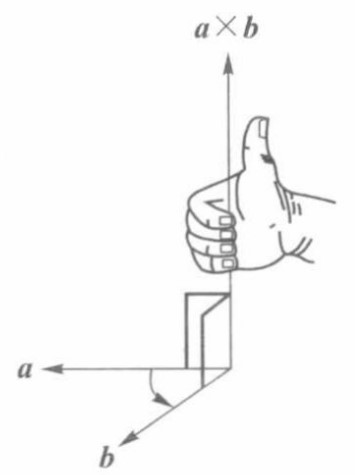
\includegraphics[width=\marginparwidth]{figures/right-hand.jpg}
	\caption{右手法则}
	\label{fig:righthand}
\end{marginfigure}

\par 向量积也称\textbf{外积}、\textbf{叉积}。

\par 向量积具有如下\textbf{基本性质}:
\begin{enumerate}
  \item \textbf{无交换律}:$\vb*{a} \times \vb*{b} = -\vb*{b} \times \vb*{a}$
  \item 分配律:$(\vb*{a}+\vb*{b}) \times \vb*{c} = (\vb*{a} \times \vb*{c})+ (\vb*{b} \times \vb*{c})$,$\vb*{a}\times(\vb*{b} + \vb*{c}) = (\vb*{a} \times \vb*{b})+ (\vb*{a} \times \vb*{c})$
  \item 关于数乘的结合律:$(k\vb*{a}) \times \vb*{b} = \vb*{a} \times (k\vb*{b})=k(\vb*{a} \times \vb*{b})$
\end{enumerate}

\par \textbf{向量积的坐标表示}:
\par 利用行列式,可以将向量积表示为:
\begin{equation}
  \vb*{a} \times \vb*{b}=
  \left |\begin{array}{ccc}
    \vb*{i} & \vb*{j} & \vb*{k} \\
    a_x     & a_y     & a_z     \\
    b_x     & b_y     & b_z     \\
  \end{array}\right |.
\end{equation}
\par 这一公式可由基向量之间的向量积关系以及向量积的分配律推导出,建议动手尝试.

\par \textbf{向量积的几何应用}:
\begin{enumerate}
  \item 判断共线:两向量$\vb*{a}$与$\vb*{b}$共线 $\Leftrightarrow$ $\vb*{a} \times \vb*{b}=0$
\end{enumerate}

\section{混合积}
\begin{definition}[混合积]
  规定三个向量$\vb*{a}$,$\vb*{b}$,$\vb*{c}$的混合积是一个数,记为$[\vb*{a} \quad \vb*{b} \quad \vb*{c}]$,$[\vb*{a} \quad \vb*{b} \quad \vb*{c}]=(\vb*{a} \times \vb*{b}) \cdot \vb*{c}$.
\end{definition}
\par 混合积具有明显的几何意义:当$\vb*{a}$,$\vb*{b}$,$\vb*{c}$成右手系时,$[\vb*{a} \quad \vb*{b} \quad \vb*{c}]$的值为如图\ref{fig:mixedproduct}平行六面体的体积.当$\vb*{a}$,$\vb*{b}$,$\vb*{c}$成左手系时,混合积的绝对值表示体积.

\par 混合积具有如下\textbf{基本性质}:
\begin{enumerate}
  \item $[\vb*{a} \quad \vb*{b} \quad \vb*{c}]=[\vb*{b} \quad \vb*{c} \quad \vb*{a}]=[\vb*{c} \quad \vb*{a} \quad \vb*{b}]$
  \item 互换混合积中任意两个向量的位置,则混合积变号.例如:$[\vb*{b} \quad \vb*{a} \quad \vb*{c}]=-[\vb*{a} \quad \vb*{b} \quad \vb*{c}]$
\end{enumerate}

\begin{marginfigure}[7em]
	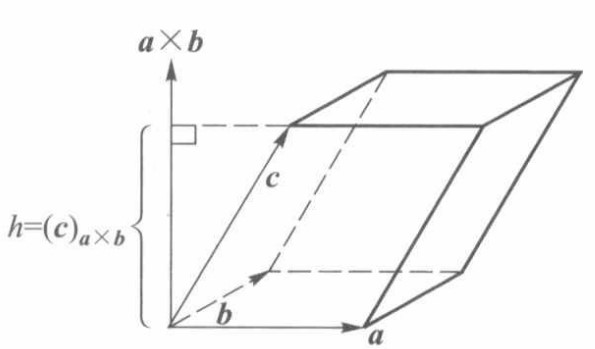
\includegraphics[width=\marginparwidth]{figures/mixed-product.jpg}
	\caption{混合积的几何意义}
	\label{fig:mixedproduct}
\end{marginfigure}

\par \textbf{混合积的坐标表示}:
\par 利用行列式,可以将混合积表示为:
\begin{equation}
  [\vb*{a} \quad \vb*{b} \quad \vb*{c}] =
  \left |\begin{array}{ccc}
    a_x & a_y & a_z \\
    b_x & b_y & b_z \\
    c_x & c_y & c_z \\
  \end{array}\right |.
\end{equation}
\par 利用这一表示,结合行列式的知识,很容易推出混合积的性质1.

\par \textbf{混合的几何应用}:

判断共面:三个向量$\vb*{a}$,$\vb*{b}$与$\vb*{c}$共面 $\Leftrightarrow$ $[\vb*{a} \quad \vb*{b} \quad \vb*{c}]=0$

\begin{example}
  求以$A(1,1,1)$,$B(2,0,1)$,$C(0,0,1)$,$D(1,3,2)$为顶点的四面体的体积$V$.
\end{example}

\begin{solution}
  $V$等于以$\overrightarrow{AB}=(1,-1,0)$,$\overrightarrow{AC}$,$\overrightarrow{AD}$为相邻棱的平行六面体的体积$\Omega$的$\frac{1}{6}$倍.再由混合积的几何意义知$\Omega$等于混合积$[\overrightarrow{AB} \quad \overrightarrow{AC} \quad \overrightarrow{AD}]$的绝对值.由于
  \begin{equation*}
    [\overrightarrow{AB} \quad \overrightarrow{AC} \quad \overrightarrow{AD}]=
    \left |\begin{array}{ccc}
      1  & -1 & 0 \\
      -1 & -1 & 0 \\
      0  & 2  & 1 \\
    \end{array}\right |
    =-2
  \end{equation*}
  故$\Omega=2$,$V=\frac{1}{3}$.
\end{solution}

\section{总结}
\begin{table}[H]
  \centering
  \caption{总结}
  \begin{tabular}{cccc}
    \toprule
           & 结果 & 几何意义         & 几何应用 \\
    \midrule
    数量积 & 数量 & 做功(物理意义) & 判断垂直 \\
    向量积 & 向量 & 平行四边形面积   & 判断共线 \\
    混合积 & 数量 & 平行六面体体积   & 判断共面 \\
    \bottomrule
  \end{tabular}
  \label{tab:summary}
\end{table}